\documentclass[varwidth=true, border=0.2cm]{standalone}
\usepackage{tikz}

\tikzset{partial ellipse/.style args={#1:#2:#3}{insert path={+ (#1:#3) arc (#1:#2:#3)}}}
\definecolor{mygreen}{RGB}{128,255,0} % original
%\definecolor{myred}{RGB}{255,128,0}   % original

%\definecolor{mygreen}{RGB}{108,211,255}
\definecolor{myred}{RGB}{255,0,0}
%\definecolor{myred}{RGB}{0,105,210} 

\begin{document}
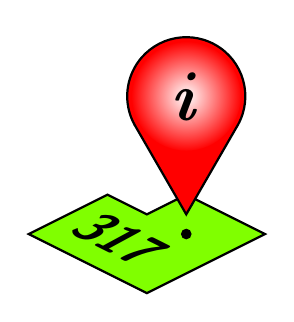
\begin{tikzpicture}

% Define grid and plot main rays
%\draw[step=.5, gray, thin, opacity=.5] (-2,0) grid (2,4);

\draw[thick,fill=mygreen] (-1.5,0.75) -- (0,0) -- (1.5,0.75) -- (0.5,1.25) -- (0,1) -- (-0.5,1.25) -- cycle;
\draw (0,0) -- (-1.5,0.75) node[above=3.5pt,pos=0.5,sloped,above,xslant=0.7] {\LARGE\textbf{\textsf{317}}};
\draw[fill=black] (0.5,0.75) circle (.06cm);

\draw[thick,fill=myred] (0.5,2.5) [partial ellipse=-29:209:.75cm and .75cm];
\draw[thick,fill=myred] (1.1595,2.143) -- (0.5,1) -- (-.1595,2.143);
%\draw[thick,fill=white] (0.5,2.5) circle (0.5cm) node {\huge{\textbf{\textit{i}}}};


\filldraw[myred,even odd rule,inner color=white,outer color=myred] (0.5,2.5) circle (0.7) (0.5,2.5) circle (0) node {\Huge{\textbf{\color{black}\textit{i}}}};

\end{tikzpicture}
\end{document}